\documentclass[%margin%,line,pifont,palatino,courier
]{article}
\usepackage{fullpage}
\usepackage{lastpage}
\usepackage[top=1in,bottom=1in,margin=1in]{geometry}
\usepackage{supertabular}
\usepackage{graphicx,tikz}	
%\usepackage{tkz-euclide}
%\usetkzobj{all}
%\usetikzlibrary{calc}
\usepackage{array,multicol}
\usepackage{amsmath,amssymb}
\usepackage{enumitem}
\usepackage{url}

\usepackage{fancyhdr}
\pagestyle{fancy}

\addtolength{\topmargin}{-0.25in}

\newcommand{\vect}[1]{\mathbf{#1}}
\DeclareMathOperator{\proj}{proj}

\fancypagestyle{plain}{
	\addtolength{\headheight}{0.485in}
	\rhead{\bf MATH 236 (Calculus II) \\
		%\vspace{0.5pc}
		due Thurs 19 Oct 2017 \\}
	\rfoot{\footnotesize THQuiz 5, p. \thepage\ (of \pageref{LastPage})
	}
\renewcommand{\headrulewidth}{0pt}
}
\fancyhf{}
\renewcommand{\headrulewidth}{0pt}
\rfoot{\footnotesize THQuiz 5, p. \thepage\ (of \pageref{LastPage})$\;$}

\title{\vspace{-3.5pc} 
	\flushleft \bf \Large Take-Home Quiz 5: Convergence of infinite sums %\\ 
	 (\S5.6, 7.3)}
\date{}

% % % % %
\begin{document}
\maketitle

\vspace{-3pc}
\noindent{\bf Directions:} This quiz is due on October 19, 2017 at the beginning of lecture.  You may use whatever resources you like -- e.g., other textbooks, websites, collaboration with classmates -- to complete it \textbf{but YOU MUST DOCUMENT YOUR SOURCES}.  Acceptable documentation is enough information for me to find the source myself.  Rote copying another's work is unacceptable, regardless of whether you document it.  

\noindent\hrulefill

\begin{enumerate}
% % %
\item Graph the function $y=x^{-1.01}$ in the first quadrant (i.e., where $x$ and $y$ are both positive).  Use limits of definite integrals to calculate the following:
	\begin{itemize}
	\item {\bf \S5.6 \#26} $\displaystyle \int_0^1 x^{-1.01}\ dx$
	\item {\bf \S5.6 \#28} $\displaystyle \int_1^{\infty} x^{-1.01}\ dx$
	\end{itemize}
	Shade the area on your graph correpsonding to the integral that converges.

% % %
\item Suppose in the course of Emmy's job as a civil engineer at Hanford, she must measure the amount of radioactive cesium present in various mixtures.  The amount of cesium (in pounds) in any particular tank $T\geq 0$ years after it is first filled is given by  
\[
Q(T)=\int_T^{\infty}ke^{-0.023t}\ dt,
\]
where $k$ is some constant.
	\begin{enumerate}
	\item {\bf \S5.6 \#71}  Suppose a particular tank was filled 12 years ago.  If Emmy measures 0.95lb of cesium in the tank now, how much cesium was in the tank when it was first filled 12 years ago? 
	\item {\bf \S5.6 \#72} In another location in the tank farm, there is a tank that was filled with a different, known mixture containing 1.5lb of radioactive cesium.  However, there is no record of when this tank was filled.  Emmy measures 0.85lb of cesium in the tank now.   How long ago was the tank filled?
	\end{enumerate} 
 
% % %
\item {\bf \S7.3 \#72} Express the repeating decimal $3.454545...$ as
	\begin{itemize}
	\item a geometric series and
	\item as a quotient of two integers reduced to lowest terms.
	\end{itemize} 

% % %
\item {\bf \S7.3 \#82} The figure shown is drawn recursively and then shaded.  The largest square has side length 1 unit.  A square whose side length is $r$\% as long as the larger square is inscribed with one vertex on each edge of the larger square.  This process is repeated recursively, resulting in shading as depicted in the figure (but goes on indefinitely).  What is the area of the shaded portion of the figure?
\begin{center}
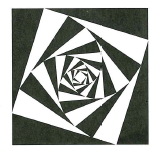
\includegraphics[scale=1.25]{7-3_82TaalmanKohn}
\end{center}

	

	
% % % % %
\end{enumerate}
\end{document}